% Options for packages loaded elsewhere
\PassOptionsToPackage{unicode}{hyperref}
\PassOptionsToPackage{hyphens}{url}
%
\documentclass[
  ignorenonframetext,
]{beamer}
\usepackage{pgfpages}
\setbeamertemplate{caption}[numbered]
\setbeamertemplate{caption label separator}{: }
\setbeamercolor{caption name}{fg=normal text.fg}
\beamertemplatenavigationsymbolsempty
% Prevent slide breaks in the middle of a paragraph
\widowpenalties 1 10000
\raggedbottom
\setbeamertemplate{part page}{
  \centering
  \begin{beamercolorbox}[sep=16pt,center]{part title}
    \usebeamerfont{part title}\insertpart\par
  \end{beamercolorbox}
}
\setbeamertemplate{section page}{
  \centering
  \begin{beamercolorbox}[sep=12pt,center]{part title}
    \usebeamerfont{section title}\insertsection\par
  \end{beamercolorbox}
}
\setbeamertemplate{subsection page}{
  \centering
  \begin{beamercolorbox}[sep=8pt,center]{part title}
    \usebeamerfont{subsection title}\insertsubsection\par
  \end{beamercolorbox}
}
\AtBeginPart{
  \frame{\partpage}
}
\AtBeginSection{
  \ifbibliography
  \else
    \frame{\sectionpage}
  \fi
}
\AtBeginSubsection{
  \frame{\subsectionpage}
}

\usepackage{amsmath,amssymb}
\usepackage{lmodern}
\usepackage{iftex}
\ifPDFTeX
  \usepackage[T1]{fontenc}
  \usepackage[utf8]{inputenc}
  \usepackage{textcomp} % provide euro and other symbols
\else % if luatex or xetex
  \usepackage{unicode-math}
  \defaultfontfeatures{Scale=MatchLowercase}
  \defaultfontfeatures[\rmfamily]{Ligatures=TeX,Scale=1}
\fi
% Use upquote if available, for straight quotes in verbatim environments
\IfFileExists{upquote.sty}{\usepackage{upquote}}{}
\IfFileExists{microtype.sty}{% use microtype if available
  \usepackage[]{microtype}
  \UseMicrotypeSet[protrusion]{basicmath} % disable protrusion for tt fonts
}{}
\makeatletter
\@ifundefined{KOMAClassName}{% if non-KOMA class
  \IfFileExists{parskip.sty}{%
    \usepackage{parskip}
  }{% else
    \setlength{\parindent}{0pt}
    \setlength{\parskip}{6pt plus 2pt minus 1pt}}
}{% if KOMA class
  \KOMAoptions{parskip=half}}
\makeatother
\usepackage{xcolor}
\newif\ifbibliography
\setlength{\emergencystretch}{3em} % prevent overfull lines
\setcounter{secnumdepth}{-\maxdimen} % remove section numbering

\usepackage{color}
\usepackage{fancyvrb}
\newcommand{\VerbBar}{|}
\newcommand{\VERB}{\Verb[commandchars=\\\{\}]}
\DefineVerbatimEnvironment{Highlighting}{Verbatim}{commandchars=\\\{\}}
% Add ',fontsize=\small' for more characters per line
\usepackage{framed}
\definecolor{shadecolor}{RGB}{241,243,245}
\newenvironment{Shaded}{\begin{snugshade}}{\end{snugshade}}
\newcommand{\AlertTok}[1]{\textcolor[rgb]{0.68,0.00,0.00}{#1}}
\newcommand{\AnnotationTok}[1]{\textcolor[rgb]{0.37,0.37,0.37}{#1}}
\newcommand{\AttributeTok}[1]{\textcolor[rgb]{0.40,0.45,0.13}{#1}}
\newcommand{\BaseNTok}[1]{\textcolor[rgb]{0.68,0.00,0.00}{#1}}
\newcommand{\BuiltInTok}[1]{\textcolor[rgb]{0.00,0.23,0.31}{#1}}
\newcommand{\CharTok}[1]{\textcolor[rgb]{0.13,0.47,0.30}{#1}}
\newcommand{\CommentTok}[1]{\textcolor[rgb]{0.37,0.37,0.37}{#1}}
\newcommand{\CommentVarTok}[1]{\textcolor[rgb]{0.37,0.37,0.37}{\textit{#1}}}
\newcommand{\ConstantTok}[1]{\textcolor[rgb]{0.56,0.35,0.01}{#1}}
\newcommand{\ControlFlowTok}[1]{\textcolor[rgb]{0.00,0.23,0.31}{#1}}
\newcommand{\DataTypeTok}[1]{\textcolor[rgb]{0.68,0.00,0.00}{#1}}
\newcommand{\DecValTok}[1]{\textcolor[rgb]{0.68,0.00,0.00}{#1}}
\newcommand{\DocumentationTok}[1]{\textcolor[rgb]{0.37,0.37,0.37}{\textit{#1}}}
\newcommand{\ErrorTok}[1]{\textcolor[rgb]{0.68,0.00,0.00}{#1}}
\newcommand{\ExtensionTok}[1]{\textcolor[rgb]{0.00,0.23,0.31}{#1}}
\newcommand{\FloatTok}[1]{\textcolor[rgb]{0.68,0.00,0.00}{#1}}
\newcommand{\FunctionTok}[1]{\textcolor[rgb]{0.28,0.35,0.67}{#1}}
\newcommand{\ImportTok}[1]{\textcolor[rgb]{0.00,0.46,0.62}{#1}}
\newcommand{\InformationTok}[1]{\textcolor[rgb]{0.37,0.37,0.37}{#1}}
\newcommand{\KeywordTok}[1]{\textcolor[rgb]{0.00,0.23,0.31}{#1}}
\newcommand{\NormalTok}[1]{\textcolor[rgb]{0.00,0.23,0.31}{#1}}
\newcommand{\OperatorTok}[1]{\textcolor[rgb]{0.37,0.37,0.37}{#1}}
\newcommand{\OtherTok}[1]{\textcolor[rgb]{0.00,0.23,0.31}{#1}}
\newcommand{\PreprocessorTok}[1]{\textcolor[rgb]{0.68,0.00,0.00}{#1}}
\newcommand{\RegionMarkerTok}[1]{\textcolor[rgb]{0.00,0.23,0.31}{#1}}
\newcommand{\SpecialCharTok}[1]{\textcolor[rgb]{0.37,0.37,0.37}{#1}}
\newcommand{\SpecialStringTok}[1]{\textcolor[rgb]{0.13,0.47,0.30}{#1}}
\newcommand{\StringTok}[1]{\textcolor[rgb]{0.13,0.47,0.30}{#1}}
\newcommand{\VariableTok}[1]{\textcolor[rgb]{0.07,0.07,0.07}{#1}}
\newcommand{\VerbatimStringTok}[1]{\textcolor[rgb]{0.13,0.47,0.30}{#1}}
\newcommand{\WarningTok}[1]{\textcolor[rgb]{0.37,0.37,0.37}{\textit{#1}}}

\providecommand{\tightlist}{%
  \setlength{\itemsep}{0pt}\setlength{\parskip}{0pt}}\usepackage{longtable,booktabs,array}
\usepackage{calc} % for calculating minipage widths
\usepackage{caption}
% Make caption package work with longtable
\makeatletter
\def\fnum@table{\tablename~\thetable}
\makeatother
\usepackage{graphicx}
\makeatletter
\def\maxwidth{\ifdim\Gin@nat@width>\linewidth\linewidth\else\Gin@nat@width\fi}
\def\maxheight{\ifdim\Gin@nat@height>\textheight\textheight\else\Gin@nat@height\fi}
\makeatother
% Scale images if necessary, so that they will not overflow the page
% margins by default, and it is still possible to overwrite the defaults
% using explicit options in \includegraphics[width, height, ...]{}
\setkeys{Gin}{width=\maxwidth,height=\maxheight,keepaspectratio}
% Set default figure placement to htbp
\makeatletter
\def\fps@figure{htbp}
\makeatother

\makeatletter
\makeatother
\makeatletter
\makeatother
\makeatletter
\@ifpackageloaded{caption}{}{\usepackage{caption}}
\AtBeginDocument{%
\ifdefined\contentsname
  \renewcommand*\contentsname{Table of contents}
\else
  \newcommand\contentsname{Table of contents}
\fi
\ifdefined\listfigurename
  \renewcommand*\listfigurename{List of Figures}
\else
  \newcommand\listfigurename{List of Figures}
\fi
\ifdefined\listtablename
  \renewcommand*\listtablename{List of Tables}
\else
  \newcommand\listtablename{List of Tables}
\fi
\ifdefined\figurename
  \renewcommand*\figurename{Figure}
\else
  \newcommand\figurename{Figure}
\fi
\ifdefined\tablename
  \renewcommand*\tablename{Table}
\else
  \newcommand\tablename{Table}
\fi
}
\@ifpackageloaded{float}{}{\usepackage{float}}
\floatstyle{ruled}
\@ifundefined{c@chapter}{\newfloat{codelisting}{h}{lop}}{\newfloat{codelisting}{h}{lop}[chapter]}
\floatname{codelisting}{Listing}
\newcommand*\listoflistings{\listof{codelisting}{List of Listings}}
\makeatother
\makeatletter
\@ifpackageloaded{caption}{}{\usepackage{caption}}
\@ifpackageloaded{subcaption}{}{\usepackage{subcaption}}
\makeatother
\makeatletter
\@ifpackageloaded{tcolorbox}{}{\usepackage[many]{tcolorbox}}
\makeatother
\makeatletter
\@ifundefined{shadecolor}{\definecolor{shadecolor}{rgb}{.97, .97, .97}}
\makeatother
\makeatletter
\makeatother
\ifLuaTeX
  \usepackage{selnolig}  % disable illegal ligatures
\fi
\IfFileExists{bookmark.sty}{\usepackage{bookmark}}{\usepackage{hyperref}}
\IfFileExists{xurl.sty}{\usepackage{xurl}}{} % add URL line breaks if available
\urlstyle{same} % disable monospaced font for URLs
\hypersetup{
  pdftitle={Grad Quant: Data Visualization {[}Day 1{]}},
  hidelinks,
  pdfcreator={LaTeX via pandoc}}

\title{Grad Quant: Data Visualization {[}Day 1{]}}
\author{}
\date{}

\begin{document}
\frame{\titlepage}
\ifdefined\Shaded\renewenvironment{Shaded}{\begin{tcolorbox}[enhanced, borderline west={3pt}{0pt}{shadecolor}, boxrule=0pt, sharp corners, frame hidden, interior hidden, breakable]}{\end{tcolorbox}}\fi

\begin{frame}{Data Visualization}
\protect\hypertarget{data-visualization}{}
\begin{itemize}
\tightlist
\item
  Data visualization is the graphical representation of information and
  data.

  \begin{itemize}
  \tightlist
  \item
    Provide an accessible way to see and understand trends, outliers,
    and patterns in data.
  \end{itemize}
\item
  Data visualization can be used for:

  \begin{itemize}
  \tightlist
  \item
    \textbf{Exploration:} Identifying and learning from patterns/trends
    in data
  \item
    \textbf{Explanation:} Explaining or communicating findings from data
  \end{itemize}
\end{itemize}
\end{frame}

\begin{frame}{Visualization in R using ggplot2}
\protect\hypertarget{visualization-in-r-using-ggplot2}{}
\begin{itemize}
\tightlist
\item
  R is increasingly adopted for statistical analyses/plotting
\item
  ggplot2 is a package within tidyverse that is most frequently used

  \begin{itemize}
  \tightlist
  \item
    Level of customization has led outlets such as BBC and NYT to adopt
    ggplot2 as their preferred data visualization tool
  \end{itemize}
\item
  Additional benefit of visualization in R (or other programming
  languages):

  \begin{itemize}
  \tightlist
  \item
    transparency
  \item
    easily adapt and re-run visualization
  \end{itemize}
\end{itemize}
\end{frame}

\begin{frame}{Grammar of Graphics}
\protect\hypertarget{grammar-of-graphics}{}
\begin{itemize}
\item
  ggplot2 plots are built in a series of layers

  \begin{figure}

  {\centering 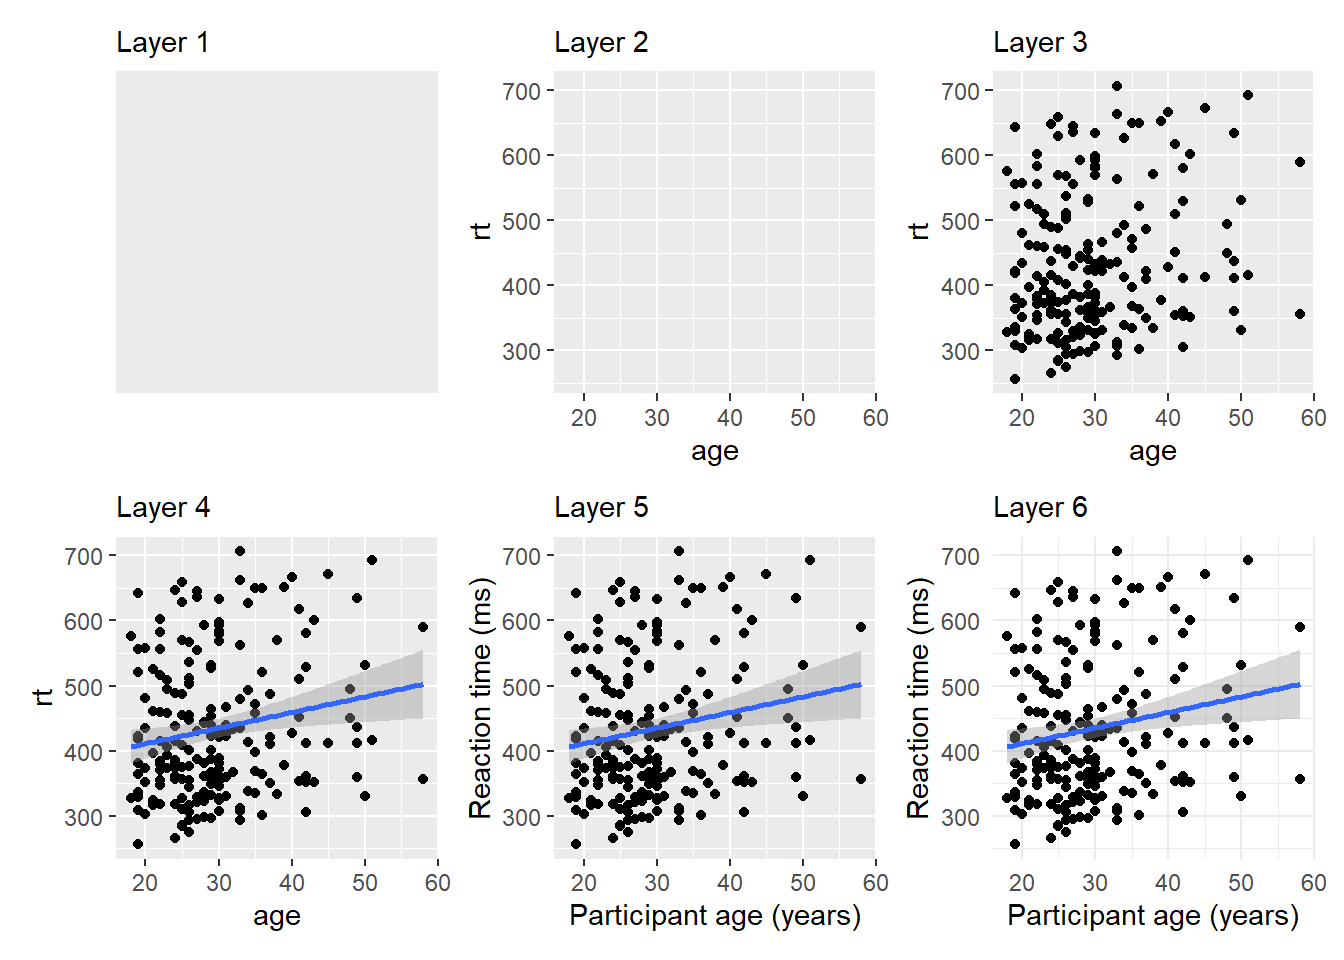
\includegraphics[width=5.20833in,height=\textheight]{https://psyteachr.github.io/introdataviz/01-ch1_files/figure-html/layers-1.png}

  }

  \caption{Evolution of a layered plot}

  \end{figure}
\end{itemize}
\end{frame}

\begin{frame}{Grammar of Graphics: Layers}
\protect\hypertarget{grammar-of-graphics-layers}{}
\begin{enumerate}
\item
  Plot space is built
\item
  The variables are specified
\item
  The type of visualisation (known as a geom) that is desired for these
  variables is specified - in this case geom\_point() is called to
  visualise individual data points;
\item
  A second geom is added to include a line of best fit, the axis labels
  are edited for readability
\item
  The axis labels are edited for readability
\item
  A theme is applied to change the overall appearance of the plot.
\end{enumerate}

These layers allow a lot of customizability by allow tweaking of layers
independently of other layers, and easy adapting of existing code.
\end{frame}

\begin{frame}[fragile]{Install Packages}
\protect\hypertarget{install-packages}{}
Run this just once, as you only need to install the package a single
time. (Well, except that you may need to update it occassionally)

\begin{Shaded}
\begin{Highlighting}[]
\CommentTok{\# install.packages("tidyverse", "patchwork")}
\FunctionTok{library}\NormalTok{(tidyverse)}
\end{Highlighting}
\end{Shaded}
\end{frame}

\begin{frame}[fragile]{Data and Descriptives}
\protect\hypertarget{data-and-descriptives}{}
Let's load the data contained in tidyverse, ``starwars'' containing data
about characters from Star Wars movies. The summary function is
contained within base R.

Let's inspect ``mass''.

\begin{Shaded}
\begin{Highlighting}[]
\FunctionTok{data}\NormalTok{(starwars)}
\FunctionTok{summary}\NormalTok{(starwars}\SpecialCharTok{$}\NormalTok{mass)}
\end{Highlighting}
\end{Shaded}

\begin{verbatim}
   Min. 1st Qu.  Median    Mean 3rd Qu.    Max.    NA's 
  15.00   55.60   79.00   97.31   84.50 1358.00      28 
\end{verbatim}
\end{frame}

\begin{frame}[fragile]
The psych package's ``desribe'' function is also helpful. The ``::''
argument allows you to call a single function from a package without
calling the full package and all of its contents.

\begin{Shaded}
\begin{Highlighting}[]
\CommentTok{\# install.packages("psych")}
\NormalTok{psych}\SpecialCharTok{::}\FunctionTok{describe}\NormalTok{(starwars}\SpecialCharTok{$}\NormalTok{mass)}
\end{Highlighting}
\end{Shaded}

\begin{verbatim}
   vars  n  mean     sd median trimmed   mad min  max range skew kurtosis    se
X1    1 59 97.31 169.46     79   75.44 16.31  15 1358  1343 6.97    48.93 22.06
\end{verbatim}
\end{frame}

\begin{frame}[fragile]
You can also do it using tidyverse approach:

\begin{Shaded}
\begin{Highlighting}[]
\NormalTok{starwars }\SpecialCharTok{\%\textgreater{}\%}
  \FunctionTok{group\_by}\NormalTok{(gender) }\SpecialCharTok{\%\textgreater{}\%}
  \FunctionTok{summarise}\NormalTok{(}
    \AttributeTok{mean =} \FunctionTok{mean}\NormalTok{(mass, }\AttributeTok{na.rm=}\NormalTok{T),}
    \AttributeTok{median =} \FunctionTok{median}\NormalTok{(mass, }\AttributeTok{na.rm=}\NormalTok{T),}
    \AttributeTok{sd =} \FunctionTok{sd}\NormalTok{(mass, }\AttributeTok{na.rm=}\NormalTok{T),}
    \AttributeTok{min =} \FunctionTok{min}\NormalTok{(mass, }\AttributeTok{na.rm=}\NormalTok{T),}
    \AttributeTok{max =} \FunctionTok{max}\NormalTok{(mass, }\AttributeTok{na.rm=}\NormalTok{T),}
    \AttributeTok{count =} \FunctionTok{n}\NormalTok{()}
\NormalTok{  )}
\end{Highlighting}
\end{Shaded}

\begin{verbatim}
# A tibble: 3 x 7
  gender     mean median     sd   min   max count
  <chr>     <dbl>  <dbl>  <dbl> <dbl> <dbl> <int>
1 feminine   54.7     55   8.59    45    75    17
2 masculine 106.      80 185.      15  1358    66
3 <NA>       48       48  NA       48    48     4
\end{verbatim}
\end{frame}

\begin{frame}[fragile]{Factors}
\protect\hypertarget{factors}{}
Maybe we want to look at some data by gender so let's ``factorize'' it:

\begin{Shaded}
\begin{Highlighting}[]
\NormalTok{starwars}\SpecialCharTok{$}\NormalTok{gender[}\DecValTok{1}\SpecialCharTok{:}\DecValTok{10}\NormalTok{]}
\end{Highlighting}
\end{Shaded}

\begin{verbatim}
 [1] "masculine" "masculine" "masculine" "masculine" "feminine"  "masculine"
 [7] "feminine"  "masculine" "masculine" "masculine"
\end{verbatim}

\begin{Shaded}
\begin{Highlighting}[]
\NormalTok{starwars }\OtherTok{\textless{}{-}} \FunctionTok{mutate}\NormalTok{(starwars, }\AttributeTok{gender =} \FunctionTok{factor}\NormalTok{(}
  \AttributeTok{x =}\NormalTok{ gender, }\CommentTok{\# column to translate}
  \AttributeTok{levels =} \FunctionTok{c}\NormalTok{(}\StringTok{"masculine"}\NormalTok{, }\StringTok{"feminine"}\NormalTok{), }\CommentTok{\# values of the original data in preferred order}
  \AttributeTok{labels =} \FunctionTok{c}\NormalTok{(}\StringTok{"masculine"}\NormalTok{, }\StringTok{"feminine"}\NormalTok{) }\CommentTok{\# labels for display}
\NormalTok{))}
\NormalTok{starwars}\SpecialCharTok{$}\NormalTok{gender[}\DecValTok{1}\SpecialCharTok{:}\DecValTok{10}\NormalTok{]}
\end{Highlighting}
\end{Shaded}

\begin{verbatim}
 [1] masculine masculine masculine masculine feminine  masculine feminine 
 [8] masculine masculine masculine
Levels: masculine feminine
\end{verbatim}
\end{frame}

\begin{frame}[fragile]{Summarize by Group}
\protect\hypertarget{summarize-by-group}{}
Let's take a look at the mass by gender:

\begin{Shaded}
\begin{Highlighting}[]
\NormalTok{psych}\SpecialCharTok{::}\FunctionTok{describeBy}\NormalTok{(starwars}\SpecialCharTok{$}\NormalTok{mass, starwars}\SpecialCharTok{$}\NormalTok{gender)}
\end{Highlighting}
\end{Shaded}

\begin{verbatim}

 Descriptive statistics by group 
group: masculine
   vars  n   mean     sd median trimmed   mad min  max range skew kurtosis
X1    1 49 106.15 184.97     80   81.08 10.38  15 1358  1343 6.31    39.82
      se
X1 26.42
------------------------------------------------------------ 
group: feminine
   vars n  mean   sd median trimmed  mad min max range skew kurtosis   se
X1    1 9 54.69 8.59     55   54.69 7.41  45  75    30 1.24     0.69 2.86
\end{verbatim}

Woah! Males have a massive standard deviation\ldots{} And it looks like
the the max is huge too. This may be a good time to inspect the data.
What would be a good way to plot this?
\end{frame}

\begin{frame}[fragile]{Histograms}
\protect\hypertarget{histograms}{}
Let's do the histogram step by step\ldots{}

Layer 1: Plot frame

\begin{itemize}
\tightlist
\item
  \texttt{data} specifies which data source to use for the plot
\end{itemize}

\begin{Shaded}
\begin{Highlighting}[]
\FunctionTok{ggplot}\NormalTok{(}\AttributeTok{data =}\NormalTok{ starwars)}
\end{Highlighting}
\end{Shaded}


\includegraphics{GQ_DataViz_Day1_files/figure-beamer/unnamed-chunk-7-1.pdf}
\end{frame}

\begin{frame}[fragile]
Layer 2: Variables specified

\begin{itemize}
\item
  \texttt{mapping} specifies which variables to map to which aesthetics
  (\texttt{aes}) of the plot. Mappings describe how variables in the
  data are mapped to visual properties (aesthetics) of geoms.
\item
  \texttt{x} specifies which variable to put on the x-axis
\end{itemize}

\begin{Shaded}
\begin{Highlighting}[]
\FunctionTok{ggplot}\NormalTok{(}\AttributeTok{data =}\NormalTok{ starwars, }\AttributeTok{mapping =} \FunctionTok{aes}\NormalTok{(}\AttributeTok{x =}\NormalTok{ mass))}
\end{Highlighting}
\end{Shaded}

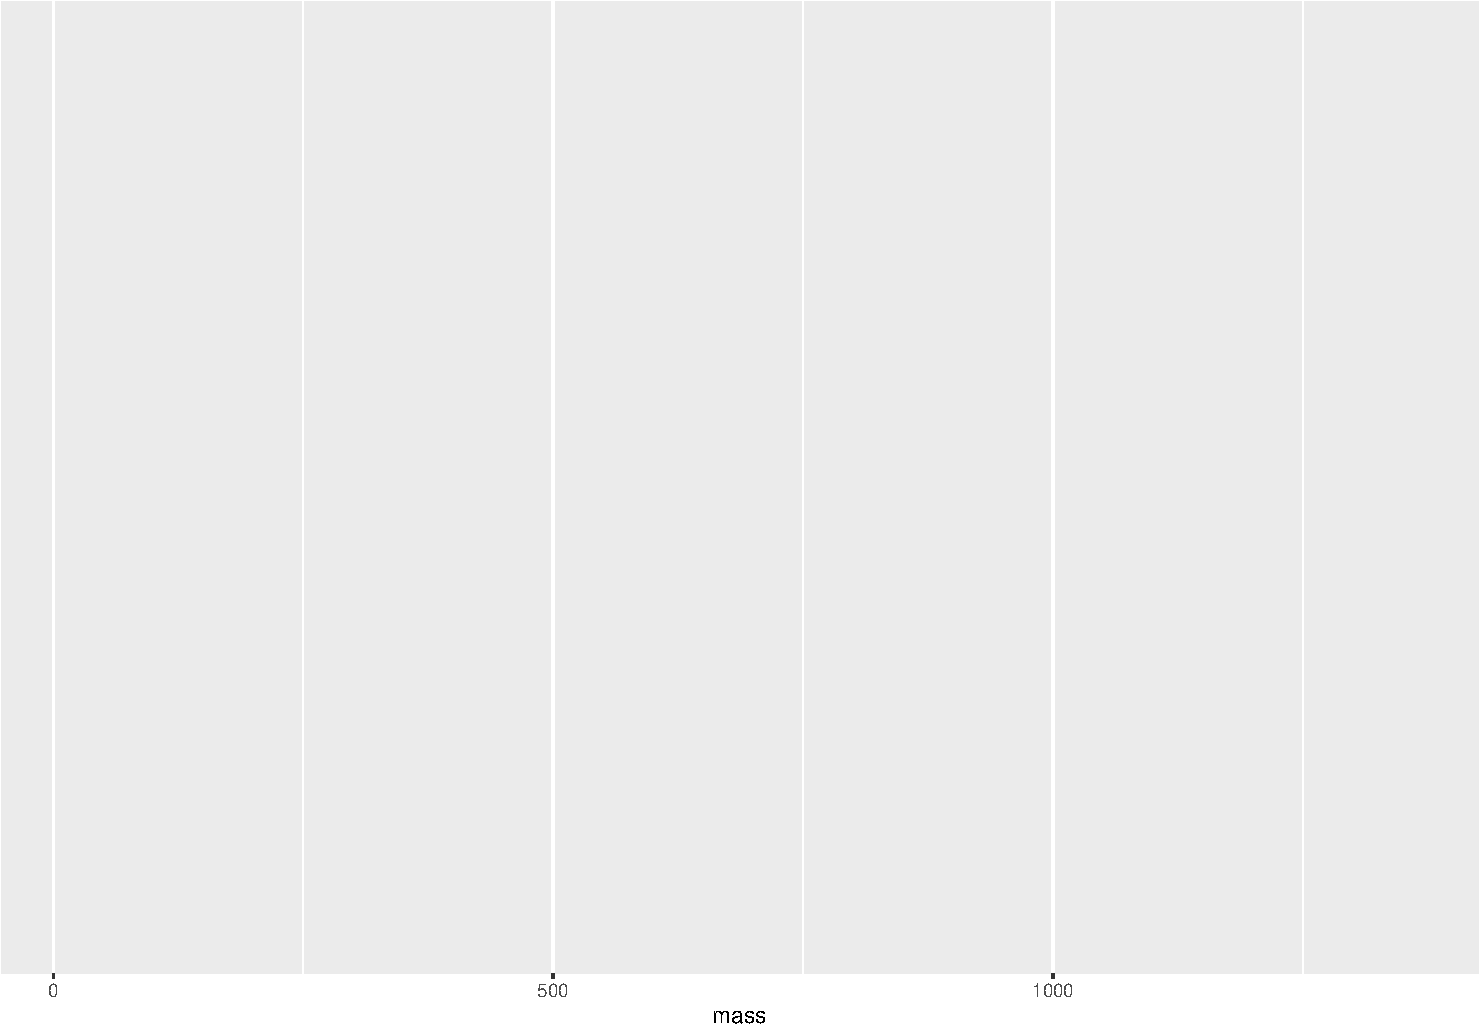
\includegraphics{GQ_DataViz_Day1_files/figure-beamer/unnamed-chunk-8-1.pdf}
\end{frame}

\begin{frame}[fragile]
Layer 3: Type of visualization.

\begin{itemize}
\tightlist
\item
  geom\_histogram() specifies that a histogram visualization will be
  used
\end{itemize}

Woah! Big outlier

\begin{Shaded}
\begin{Highlighting}[]
\FunctionTok{ggplot}\NormalTok{(}\AttributeTok{data =}\NormalTok{ starwars, }\AttributeTok{mapping =} \FunctionTok{aes}\NormalTok{(}\AttributeTok{x =}\NormalTok{ mass)) }\SpecialCharTok{+} \FunctionTok{geom\_histogram}\NormalTok{()}
\end{Highlighting}
\end{Shaded}

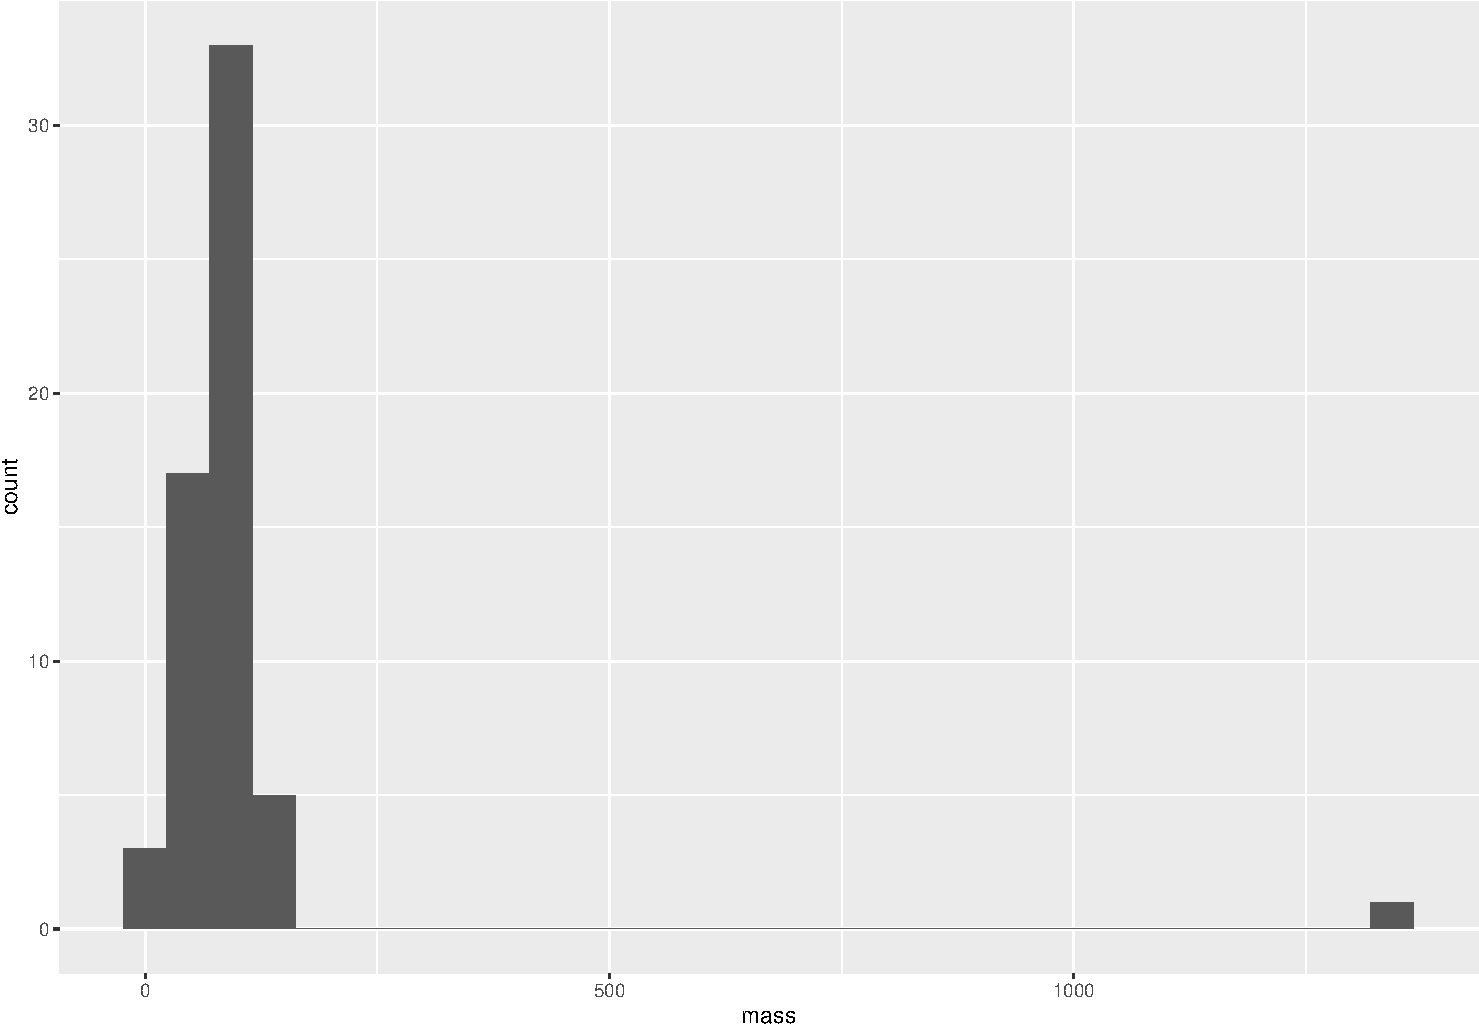
\includegraphics{GQ_DataViz_Day1_files/figure-beamer/unnamed-chunk-9-1.pdf}
\end{frame}



\end{document}
